\documentclass[12pt]{article}

\usepackage{amsmath,amsfonts,amsthm,amssymb}
\usepackage{color}
\usepackage{graphicx}
\usepackage{wrapfig}
\usepackage{epsfig}
%\usepackage{subfigure}
\usepackage{times}
\usepackage{xspace}
\usepackage{url}
\usepackage{pdfpages}
\usepackage{array}
\usepackage{subfig}
\usepackage{multirow}
\usepackage{dblfloatfix} 

\setlength{\topmargin}{0.0in}     % top of paper to head (less one inch)
\setlength{\headheight}{0in}      % height of the head
\setlength{\headsep}{0in}         % head to the top of the body
\setlength{\textheight}{9.0in}    % height of the body
\setlength{\oddsidemargin}{-.25in} % left edge of paper to body (less one inch)
\setlength{\evensidemargin}{0mm}  % ditto, even pages
\setlength{\textwidth}{7.0in}     % width of body
\setlength{\topskip}{0in}         % top of body to bottom of first line of text
\setlength{\parindent}{1pc}       

\begin{document}
\thispagestyle{empty}
%%%%%%%%%%%%%%%%%%%%%%%%%%%%%%%%%%%%%%%%%%%%%%%%%%%%%%%%%%%%%%%%%%%%%%%%%%%%%%%%%%%%%%%%
% Project Summary
%%%%%%%%%%%%%%%%%%%%%%%%%%%%%%%%%%%%%%%%%%%%%%%%%%%%%%%%%%%%%%%%%%%%%%%%%%%%%%%%%%%%%%%%
\begin{center}
{\Large\bf Assignment \#4: Data Collection and Preparation}
\vspace{3mm}
\\Caitlin Ross \& Noah Wolfe
\\02/18/2016
\\*[3mm]
\end{center}
%%%%%%%%%%%%%%%%%%%%%%%%%%%%%%%%%%%%%%%%%%%%%%%%%%%%%%%%%%%%%%%%%%%%%%%%%%%%%%%%%%%%%%%%
% Task Objects
%%%%%%%%%%%%%%%%%%%%%%%%%%%%%%%%%%%%%%%%%%%%%%%%%%%%%%%%%%%%%%%%%%%%%%%%%%%%%%%%%%%%%%%%
\section{Data Source (ROSS)}
%Description of the data source and corresponding applications.
In this assignment, we have decided to generate/collect data from our ROSS research projects. 
ROSS is a massively parallel discrete-event simulator that
can process billions of events per second \cite{Holder}, \cite{Bauer}. ROSS
models are made up of a collection of logical processes (LPs).
Each LP models a distinct component of the system. LPs
interact with one another through events in the form of time-stamped messages. An MPI task is abstracted as a processor
element (PE) in ROSS. Each PE owns a number of LPs and
schedules events in time-stamp order for all LPs assigned to
it. Events that are destined for a logical process on another
PE (i.e. remote events) are sent as MPI messages. 

For parallel execution, ROSS uses an optimistic synchronization protocol.  When an LP determines it has processed events out of timestamp order, it rolls back event computation and re-executes events in the correct order.  The Global Virtual Time (GVT) is computed on a regular basis, which allows for a reclamation of events with timestamps smaller than GVT.  The ROSS scheduler computes GVT every \texttt{gvt\_interval} iterations in the scheduling loop.  Another variable \texttt{batch} can be set to determine the number of events processed during each iteration of the scheduling loop, so \texttt{gvt\_interval$*$batch} events are processed between successive GVT computations.  Changing these parameters can trigger large changes in metrics such as number of reverse computations, remote events, event efficiency, etc. Currently, the only data collection is averaged over all processes and collected at the very end of the simulation. 

\section{Research Questions} \label{questions}
%Write down at least 2 specific research questions that can be solved by analyzing this data. The first should be "obvious" and may simply communicate the overall quantity of data you've got your hands on. The second should be more complex or subtle, that can be answered by the data, but will involve rearranging or simplifying or finding correlations within the data.

ROSS is designed to be a very fast and efficient simulator. In order to get the best possible speed-up, developers need to know what is going on behind the curtains throughout the simulation. We need to know not only if a simulation is experiencing hotspots, but also be able to detect the cause of those hotspots. This requires collection of data throughout the simulation. Two research questions that can be solved by analyzing ROSS runtime system data are:

\begin{itemize}
  \item Where is my simulation spending it's compute time?
  \item Which metrics are most influenced by the \texttt{batch} and \texttt{gvt\_interval} parameters?
\end{itemize}

The first research question should be answerable by simply visualizing the large set of collected data. 
The second item will require much more data manipulation and analysis such as a weighting system to find correlations between ROSS parameters and simulation speed.

\section{Hypotheses}
%What are your specific hypotheses related to these research questions? What knowledge are your drawing on to make these predictions?

The results to the above research questions are very dependent on the given model so we will focus on using the Slim Fly network model which simulates a large cluster of compute nodes connected and communicating in a Slim Fly topology. Simulating a uniform random workload and using the minimal routing algorithm, we expect to see the majority of the simulation compute time being spent performing forward events. This hypothesis comes from prior knowledge of the mapping of LPs to PEs for the Slim Fly model in ROSS. A uniform distribution of compute nodes, routers, and MPI processes means work should be evenly distributed and result in very little rollback activity. In the case of the second research question, we expect to find that the \texttt{batch} size parameter has the most influence on limiting remote events. This prediction is based on prior experience playing with the batch size to minimize execution time.

\section{Data Format, Extraction \& Manipulation} 
%With your research questions in mind, design the detailed format for your raw data (the columns of your data "spreadsheet") and decide on the action or sampling frequency for each "row" of the data. Make sure you are able to acquire an "interesting" amount of data, both number of samples (at least 1000 rows?) and dimensions per sample (at least 3 columns?) Note: These estimates are not requirements. If your data has many more columns, things can be quite interesting even with far fewer rows.
%Detail the efforts you made to collect, parse, reorganize, simplify, and/or post-process this data source.

Using the simple csv format, the raw data is structured so that the columns represent the various ROSS parameters and metrics and the rows represent those same parameters collected at a later instance of simulation time. The default sampling frequency is $0.01*$\texttt{simulation\_end\_time} but can be adjusted with a command line flag \texttt{--report-interval=$n$} where $n\in \{0.999, ..., 1/simulation\_end\_time\}$. Each MPI process creates its own data file and appends the MPI rank number to the end of the filename. Filenames can be adjusted with the command line flag \texttt{--stats-filename=string}. We are currently collecting a total of 20 ROSS simulation metrics (20 columns) and can sample up to 50,000 points in time for 4 MPI processes. This configuration results in 4 million data points. Even larger data sets can be generated with longer simulation runtimes.

The results we show here are from Slim Fly model runs where we vary either the \texttt{•}xttt{batch} or \texttt{gvt\_interval} parameters.  We perform experiments where \texttt{batch} is held constant at 8 and \texttt{gvt\_interval} varies from 2 to 1024 by powers of 2.  We also perform experiments where \texttt{gvt\_interval} is held constant at 8 and \texttt{batch} varies from 2 to 128 by powers of 2.  


\section{Sample Visualizations}
%Create (at least 2) simple visualization plots of this data using a tool that's new to you (or you would like to learn more about). Consider using: Excel, LineUp, Tableau, Google Analytics, Plotly, or VTK. These plots should attempt to answer the research questions you posed earlier. You can revise your research questions as needed as you work with the data.

The first visualization shown in Figure \ref{Area}, was created using the Plotly \cite{Plotly} web-based visualization tool and is used to answer the first research question posed in section \ref{questions}. The figure displays the total events computed in the simulation as well as the number of events computed for specific event types such as rollbacks, fossil collection, etc. As can be seen in the figure, the number of All Reduce computations exceeds all other types of computation so it appears the majority of the time is spent performing MPI\_All\_Reduce. 

To answer the second research question, we decided to visualize our data using a parallel coordinates graph.  We decided to use d3 again for this, as we found a very easy to use parallel coordinates library~\cite{Chang} that is built on top of d3.js.  The graphs are also hosted at \url{http://homepages.rpi.edu/~rossc3/parcoords.html}. We were able to use this d3.parcoords library to easily add interactive features, such as selecting a range on any number of axes as well as being able to shuffle the axes. Hovering over the axis names and scrolling with a mouse will also rotate the names so that they're easier to read.  The first axis in both graphs show either the value for \texttt{batch} or \texttt{gvt\_interval} and all other columns are the same between both graphs.  Each line is a result for a GVT computation for a PE in a given simulation run.  All lines for a given \texttt{batch} or \texttt{gvt\_interval} value are given the same color.  For example, in Figure \ref{fig:batch}, all data points, regardless of GVT computation and PE, are colored yellow for \texttt{batch=128}.

Figure \ref{fig:batch} shows the parallel coordinates graph for the various \texttt{batch} values and Figure \ref{fig:gvt} shows the graph for various \texttt{gvt\_interval} values.  Some metrics had values of 0 for all data points, so we removed those metrics from the graphs, leaving 15 metrics.   \texttt{batch} has the most influence on total number of events processed, events rolled back, primary and secondary roll backs,  efficiency, and remote sends and receives.  These metrics are interrelated. For instance, efficiency is based on the ratio of roll backs to total events.  As there are more rollbacks, efficiency is lower because the simulation is spending more time processing reverse events over forward events.  \texttt{gvt\_interval} does not affect total events processed and number of events rolled back as much as the \texttt{batch} parameter (Note that the scales are different between the batch and gvt-interval graphs).  Because of this, efficiency is less affected for the different \texttt{gvt\_interval}.  
\begin{figure}[!ht]
     \centering
     \subfloat[][Overall View]{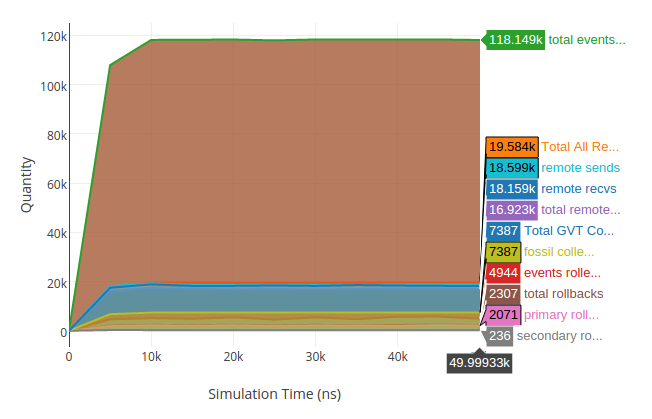
\epsfig{file=figures/area1.png, height=2.0in, width=3.00in}\label{left}}
     \subfloat[][Dense Section Zoomed View]{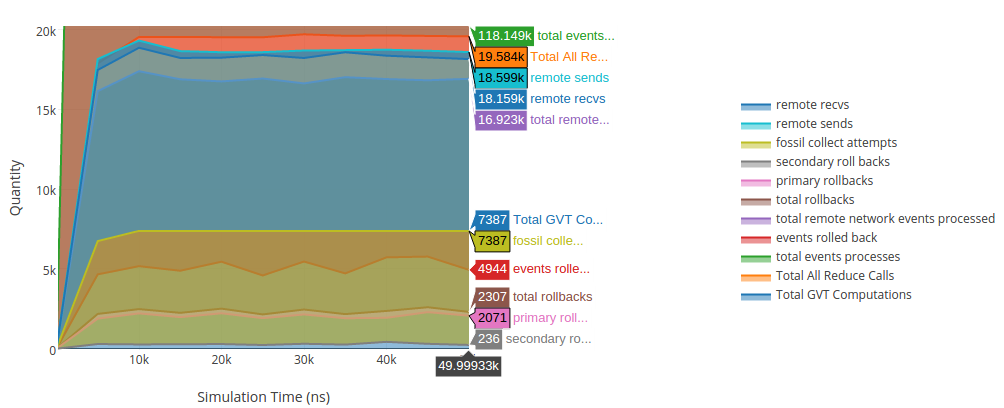
\epsfig{file=figures/area2.png, height=2.0in, width=4.50in}\label{right}}
     \caption{Visualizations of the ROSS data set showing the number of events computed in each section of the simulation over the length of the simulation. Sub-figure \ref{left} shows a global view of all metrics while sub-figure \ref{right} shows a view zoomed in on the dense region at the bottom of sub-figure \ref{left}.}
     \label{Area}
\end{figure}

\begin{figure}[ht]
\centering
	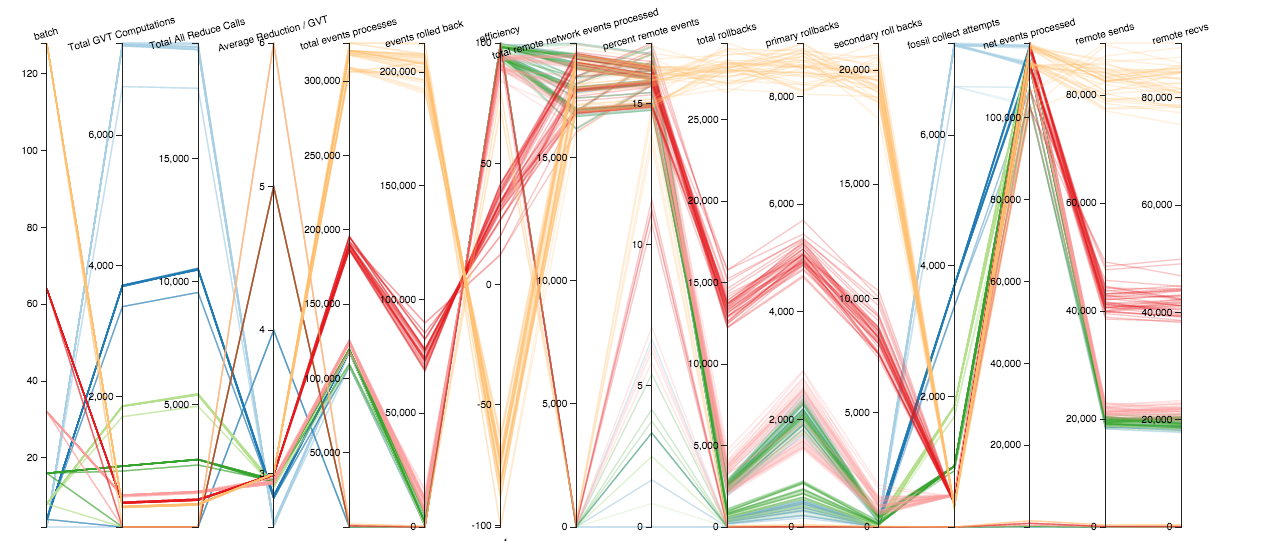
\includegraphics[width=7in]{figures/batch.png}
\caption{Parallel Coordinates graph for runs with various batch values}
\label{fig:batch}
\end{figure}
\begin{figure}[ht]
\centering
	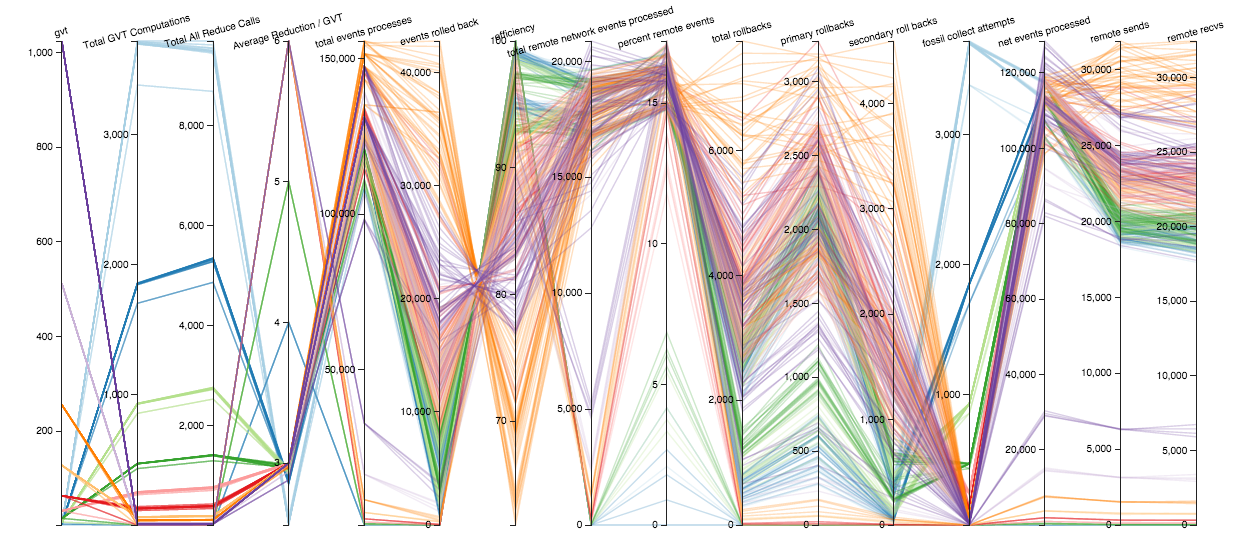
\includegraphics[width=7in]{figures/gvt.png}
\caption{Parallel Coordinates graph for runs with various gvt-interval values}
\label{fig:gvt}
\end{figure}

\section{Visualization Tool Review}
%A brief review of the tool you used to create the visualizations.
As mentioned before, we used Plotly to generate the area plot visualizations of the dataset. Plotly is a web based utility that also has support and APIs for non web based applications such as Excel, Matlab and programming languages like R and python. Overall, Plotly is a very user friendly and easy to use tool for creating relatively dynamic visualizations. The interface is very similar to an excel worksheet and allows you to import data from file or create and manipulate data within the worksheet. Plotly also has a large selection of visualization types from ugly simple pie charts to complex heat maps and large sets of interaction capabilites. The Plotly vis tool also appears to have no issues with handling large data sets. The one downfall for the software is the control over the visualizations. After you select the type of visualization you want, the amount of customization is very limited. Perhaps there is more customization if you use the API with python or another language. 

The d3.parcoords.js library used made the creation of the parallel coordinates graph very simple.  Before finding this library, we tried to edit an example that used d3.js only, but it was very difficult for us to figure out how to get the various colors set for each grouping of batch or gvt\_interval data points.  Once we found this library, it was very simple to add in color, as well as the interactive aspects (axis shuffling and selection of a subset of the data).  However, we still had difficulty with trying to change the scales of the axes.  The current setup just bases it on the data, but it would be more helpful to match the axes between the two different graphs so that each metric has the same scale on both graphs.  

% Bibliography
\bibliographystyle{abbrv}
\bibliography{HW4}

\end{document}


%\begin{figure}[!ht]
%     \centering
%     \subfloat[][twopi]{\epsfig{file=figures/MMS7-3-17.png, height=2.2in, width=4.80in}\label{vis-100-1}}\\
%     \subfloat[][dot]{\epsfig{file=figures/MMS7-3-12.png, height=2.0in, width=3.00in}\label{vis-100-2}}
%     \subfloat[][circo]{\epsfig{file=figures/MMS7-3-circo.png, height=2.0in, width=3.0in}\label{vis-100-3}}\\
%     \caption{Visualizations of the class social network data using a collection of Graphviz graph drawing programs. Red lines represent "before RPI" connections, blue represent "lived with" connections and black represent "Data Structures" connections. }
%     \label{vc-occupancy}
%\end{figure}

%\begin{figure}[!h]
%\centering
%\epsfig{file=figures/storyboard.jpg, width=5.5in}
%\caption{Storyboard showing the desired layout and interaction of the network visualization tool in D3.}
%\label{good}
%\end{figure}